% THIS IS SIGPROC-SP.TEX - VERSION 3.1
% WORKS WITH V3.2SP OF ACM_PROC_ARTICLE-SP.CLS
% APRIL 2009
%
% It is an example file showing how to use the 'acm_proc_article-sp.cls' V3.2SP
% LaTeX2e document class file for Conference Proceedings submissions.
% ----------------------------------------------------------------------------------------------------------------
% This .tex file (and associated .cls V3.2SP) *DOES NOT* produce:
%       1) The Permission Statement
%       2) The Conference (location) Info information
%       3) The Copyright Line with ACM data
%       4) Page numbering
% ---------------------------------------------------------------------------------------------------------------
% It is an example which *does* use the .bib file (from which the .bbl file
% is produced).
% REMEMBER HOWEVER: After having produced the .bbl file,
% and prior to final submission,
% you need to 'insert'  your .bbl file into your source .tex file so as to provide
% ONE 'self-contained' source file.
%
% Questions regarding SIGS should be sent to
% Adrienne Griscti ---> griscti@acm.org
%
% Questions/suggestions regarding the guidelines, .tex and .cls files, etc. to
% Gerald Murray ---> murray@hq.acm.org
%
% For tracking purposes - this is V3.1SP - APRIL 2009

\documentclass{acm_proc_article-sp}
\usepackage{graphicx}
\usepackage{hyperref}
\usepackage{csquotes}
\graphicspath{ {images/} }

\begin{document}

\title{Designing Tools and Activities for Data Literacy Learners}
\subtitle{[Short Paper]}

\numberofauthors{2} 
\author{
\alignauthor
Rahul Bhargava\\
       \affaddr{MIT Center for Civic Media}\\
       \affaddr{20 Ames St.}\\
       \affaddr{Cambridge, MA 02142, USA}\\
       \email{rahulb@mit.edu}
\alignauthor
Catherine D'Ignazio\\
       \affaddr{Emerson Engagement Game Lab}\\
       \affaddr{160 Boylston St. (4th floor)}\\
       \affaddr{Boston, MA 02116, USA}\\
       \email{catherine\textunderscore dignazio@emerson.edu}
}

\date{17 May 2015}

\maketitle
\begin{abstract}
Data-centric thinking is rapidly becoming vital to the way we work, communicate and understand in the 21st century. This has led to a proliferation of tools for novices that help them operate on data to clean, process, aggregate, and visualize it. Unfortunately, these tools have been designed to support \emph{users} rather than \emph{learners} that are trying to develop strong data literacy. This paper outlines a basic definition of data literacy and uses it to analyze the tools in this space. Based on this analysis, we propose a set of pedagogical design principles to guide the development of tools and activities that help learners build data literacy. We outline a rationale for these tools to be strongly \emph{focused}, well \emph{guided}, very \emph{inviting}, and highly \emph{expandable}. Based on these principles, we offer an example of a tool and accompanying activity that we created. Reviewing the tool as a case study, we outline design decisions that align it with our pedagogy. Discussing the activity that we led in academic classroom settings with undergraduate and graduate students, we show how the sketches students created while using the tool reflect their adeptness with key data literacy skills based on our definition.  With these early results in mind, we suggest that to better support the growing number of people learning to read and speak with data, tool designers and educators must design from the start with these strong pedagogical principles in mind.
\end{abstract}

\section{Introduction}

There is a large and growing body of literature arguing that working with data is a key modern skill.  The position of data scientist is rapidly becoming a necessary and respected role in the corporate world \cite{patil_data_2012}.  Data-driven journalism is widely regarded as a core future proficiency for the news industry \cite{howard_art_2014}.  A growing movement to make data-driven decisions in government is spurring a call for greater engagement and education with the public \cite{gurstein_open_2011,philip_framework_2013}.  

Responding to this, there are many efforts underway to build data literacy among the general public and among specific communities. Popular press has argued for broad data literacy education \cite{harris_data_2012,maycotte_data_2014}. Workshops for non-profits and activists throughout the world are introducing tools and documenting best practices that can help use data to advocate for change \cite{_visualizing_2014}.

However, there is a lack of consistent and appropriate approaches for helping novices learn to \enquote{speak data}.  Some approach the topic from a math- and statistics-centric point of view, aligning themselves with core curricular standards in public education systems \cite{maine_2015}. Some build custom tools to support intentionally designed activities based on strong pedagogical imperatives \cite{williams_city_2015}. Still others have brought together diverse communities of interested parties to build documentation, trainings, and other shared resources in an effort to grow the \enquote{movement}\cite{gray_data_2012}.

\subsection{What is Data Literacy?}

These approaches share some basic tenets of \enquote{data literacy}. Their historical roots are found in the fields of mathematics, data mining, statistics, graphic design, and information visualization \cite{fry_computational_2004}. Early academic efforts to define data literacy were linked to previous traditions in information literacy and statistical literacy \cite{schield_information_2004,hunt_challenges_2004}.  Current approaches share a hierarchical definition involving identifying, understanding, operating on, and using data.  However, while some focus on understanding and operating on the data, others focus on putting the data into action to support a reasoned argument \cite{deahl_better_2014}.

Building on these existing descriptions, we adopt a multi-faceted definition of data literacy.  For our purposes, data literacy includes the ability to read, work with, analyze and argue with data. \textbf{\textit{Reading}} data involves understanding what data is, and what aspects of the world it represents. \textbf{\textit{Working with}} data involves creating, acquiring, cleaning, and managing it. \textbf{\textit{Analyzing}} data involves filtering, sorting, aggregating, comparing, and performing other such analytic operations on it. \textbf{\textit{Arguing with}} data involves using data to support a larger narrative intended to communicate some message to a particular audience.

\section{Existing Approaches}

There have been a wide variety of approaches to building data literacy. Some tool-designers in the computer science field have focused on developing technologies that focus on building the mappings needed to translate numbers into representative visuals \cite{huron_constructive_2014}. Others have situated data collection and evidence-based argument in real local issues that connect to the learners' lived experience \cite{williams_city_2015}.  Arts-based activities have been used as an introduction to information in an attempt to bring a playful approach to working with data \cite{bhargava_data_2015}. Still others use a role-based team-building approach to build the multi-disciplinary teams needed to work with and argue with data \cite{school_2015}.

Within this context there has been, and continues to be, a proliferation of tools created to assist novices in gathering, working with, and visualizing data. These tools have been carefully cataloged and reviewed \cite{_visualizing_2014,othman_netstories_2015}, but there has been little discussing of \emph{why} and \emph{when} to use these tools in appropriate ways for the learners that do not yet \enquote{speak data}.

In addition, these tools currently focus on outputs (spreadsheets, visualizations, etc), and not on the ability to help novices learn.  Visualizations, which garner so much popular media and social media attention, are the outputs of a process. These flashy pictures attract the bulk of the attention, which has led tool designers to prioritize features that quickly create strong visuals, at the expense of tools that scaffold a process for learners.

\subsection{Defining the Tool Space}

We propose evaluating this tool space on axes of  \textbf{\textit{learn-ability}} and \textbf{\textit{flexibility}} as a useful exercise to support the argument that tools haven't focused on learning experiences.  An easy-to-learn tool is designed to be easy to use for novices that do not have any experience with it.  A hard-to-learn tool takes significant effort and commitment on the part of the learner to master it.  A flexible tool allows the user to create many types of outputs.  An inflexible tool is well-suited for creating just one type of output.

\begin{figure}[h]
\caption{Informally mapping out some data tools to compare learn-ability and flexibility}
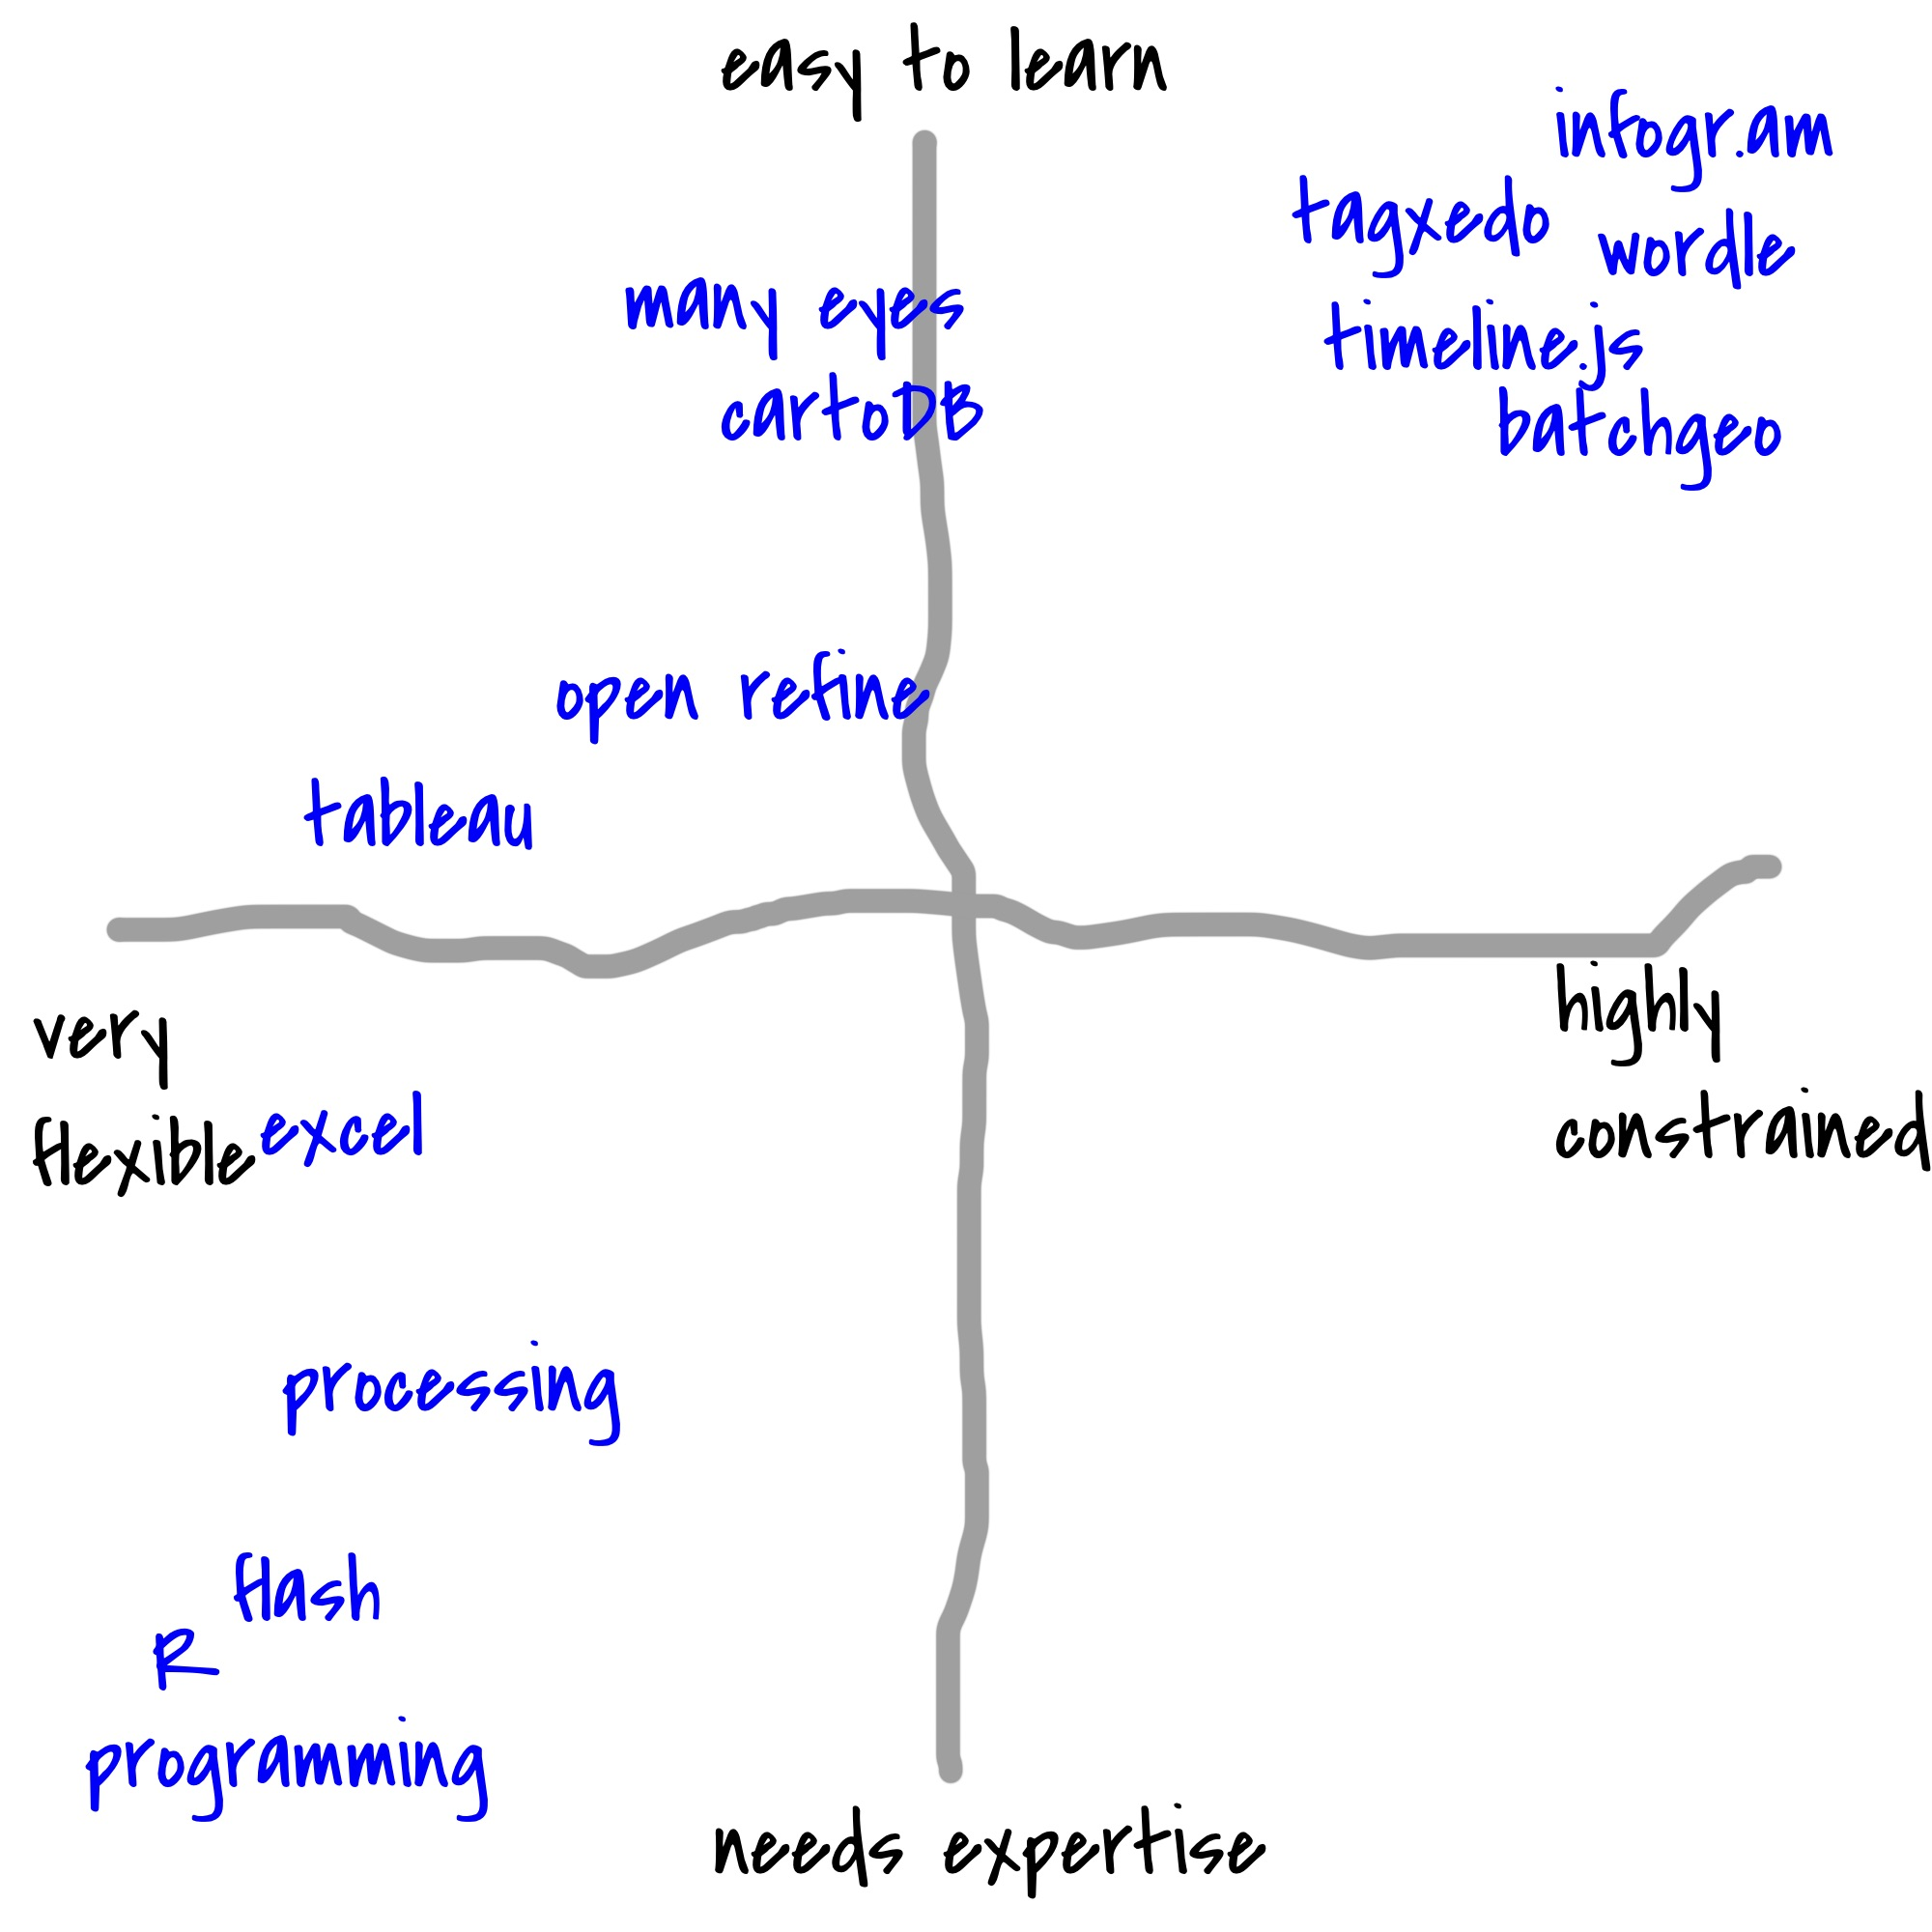
\includegraphics[width=\linewidth]{tool-matrix}
\label{fig:tool-matrix}
\end{figure}

Figure \ref{fig:tool-matrix} maps out a selection of tools in this space with learn-ability on the vertical axis and flexibility on the horizontal axis. Our informal analysis suggests that tool designers have focused on easy-to-learn tools that do just one thing (i.e. the upper right quadrant).  These tools that are easy to learn could be mistaken for tools that focus on learners, but they are not one and the same. To tease out the differences, we must analyze the pedagogical approaches of the tools in this upper-right quadrant.

\section{Pedagogical Approaches}

We propose that the pedagogical approach to building tools for data literacy learners should pull from the rich histories of traditional literacy education and designing computational tools for learning.

Traditional approaches to building reading and writing abilities have many models for building literacy. Since our definition of data literacy includes a call to reason and argue with data, we follow in the footsteps of traditional literacy models that focus on connecting literacy to argument and action.  Here Paulo Freire's approach to contextualizing literacy in the issues, settings, and topics that matter to the learner is highly relevant \cite{freire_pedagogy_1968}.  This empowerment-focused pedagogy transfers well to the domain of designing activities to build  data literacy.  Drawing inspiration from elements of Freire's \emph{popular education}, an educational approach emphasizing critical thinking and consciousness, we suggest that data literacy tools need to be introduced with activities that are inclusive, use data that are relevant to the learner, and be open to creating unexpected outputs.

In the domain of designing computational tools for learning, the discourse is quite varied in regards to approaches and how to tailor designs for learning experiences. In this field we find inspiration in Seymour Papert's approach to building \enquote{microworlds}, suggesting that key metaphors in learning tools be resonant with learners and that constraints be carefully selected to provide a rich-enough, but not too-rich, environment \cite{papert_mindstorms:_1980}. Applications of this pedagogy tend to support incremental learning, allowing novices to explore more complex aspects of the topic or tool as they increase their ability \cite{dasgupta_learning_2012,huron_constructive_2014}, and hold up the concept of teacher as facilitator, guiding learners as they explore new topic areas to construct meaningful artifacts \cite{deahl_better_2014}.

With this pedagogical history in mind, we argue that a tool that is easy to learn is not necessarily designed to support rich learning. Unless the tool and its accompanying activities implement these principles in some way, they are missing an opportunity to help the user grow their data literacy. Many of the tools in the easy-to-learn/do-one-thing quadrant introduce themselves as \enquote{magic}, explicitly hiding the mental models and software operations that they run through to produce their outputs. This pedagogy suggests the tool should be designed to make these operations more transparent, so the learner can begin to understand the conceptual language and processes of the field.

\subsection{Design Principles}

How do data tools go about implementing this pedagogical approach?  Synthesizing these rich pedagogical traditions, we propose that data literacy tools and activities that support learners must be \textbf{\textit{focused}}, \textbf{\textit{guided}}, \textbf{\textit{inviting}}, and \textbf{\textit{expandable}}.  

A \textbf{\textit{focused}} tool strives to do one thing well.  These tools sit in the previously mentioned easily learn-able and inflexible upper-right quadrant of our tool space.  Focused tools do not provide many types of options, and thus can provide a low barrier to entry for data literacy learners.  They create a small playground that is rich enough for the learner to play within, but not so rich that they get lost.

A \textbf{\textit{guided}} tool is introduced with strong activities to get the learner started.  Blank-slate websites require novice users to imagine usage scenarios.  Guided tools combat this by introducing themselves with an activity that holds the learner's hand as they get started.  These tools might immediately present an on-ramp for learners via example data and example outputs.

An \textbf{\textit{inviting}} tool is introduced in a way that is appealing to the learner. This might involve using data on a topic that is relevant or meaningful to them, or simply using humor and playfulness to invite the learner to experiment.  Inviting tools make conscious decisions about user interface and copy-writing to offer a consistent, appealing, and non-intimidating invitation to the learner. Inviting activities use familiar materials to produce playful outputs that attract interest and excitement from learners.

An \textbf{\textit{expandable}} tool is appropriate for the learner's abilities, but also offers them paths to deeper learning.  They overcome a single-minded focus by including call-outs and capabilities that allow the learner an opportunity and pathway to learn more about how the tool works.  Expandable tools recognize that they are steps along the path to building stronger data literacy for the learner, and help bridge from previous work to next steps.

We propose these design principles as a set of strong criteria to use when designing new tools and activities for data literacy learners.

\section{Case Study}

To demonstrate and evaluate these design principles in action, we created and tested a new tool for data literacy learners in the undergraduate and graduate academic setting. The academic courses we tested this tool in, along with others that teach data journalism \cite{willis_text_2015}, introduce the idea that unstructured text can be analyzed in systematic ways. Despite the previously mentioned breadth of new tools for data novices, few exist for basic quantitative text analysis. To perform a simple task such as counting the most frequent words and phrases in a text corpus, students are usually required to learn a programming language and use 3rd party software libraries \cite{bird_natural_2009}! To address this we developed a simple web-based tool and an accompanying activity to introduce quantitative text analysis to students in our classes.

\subsection{A Tool for Quantitative Text Analysis}

\begin{figure}[h]
\caption{WordCounter - A simple tool to introduce quantitative text analysis}
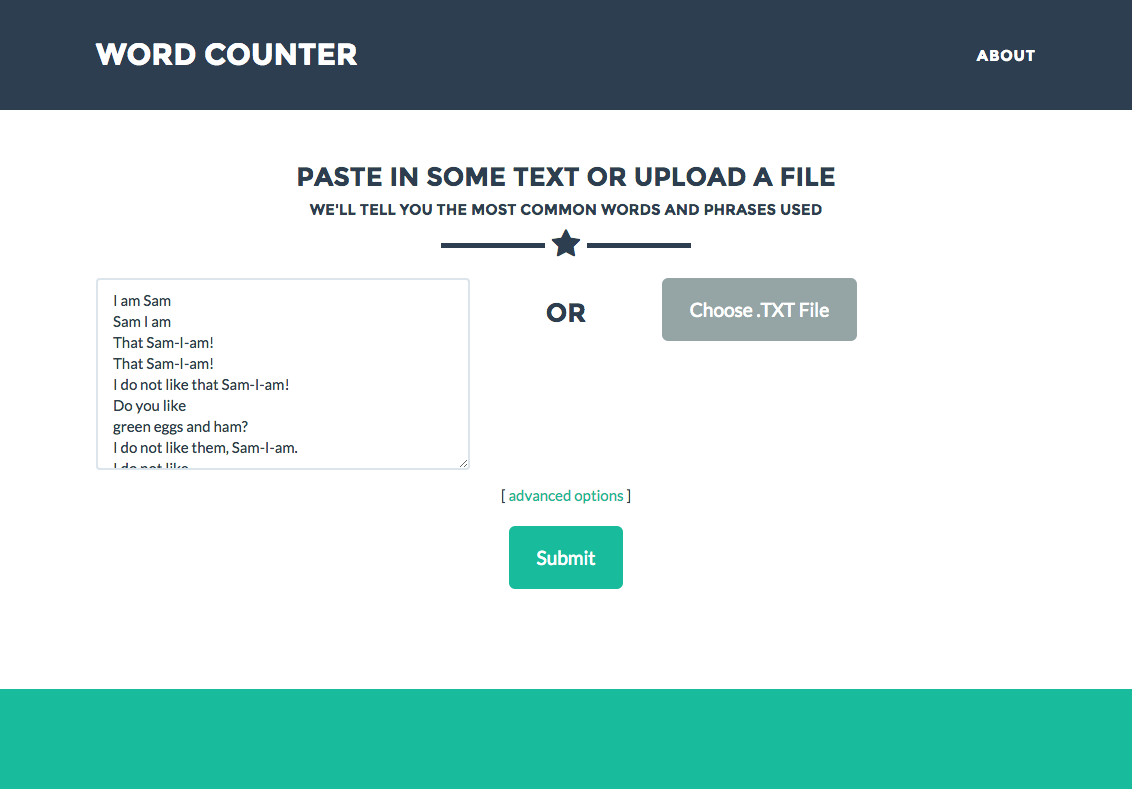
\includegraphics[width=\linewidth]{wordcounter}
\label{fig:wordcounter}
\end{figure}

WordCounter (Figure \ref{fig:wordcounter}) is a simple web application in which users can paste a block of text or upload a plain text file. The back-end server uses libraries to count the words, bigrams (two-word phrases) and trigrams (three-word phrases) in the uploaded text. After submitting their corpus, the user sees tables listing the most frequency used words, bigrams, and trigrams along with an option to download a CSV file (Figure \ref{fig:wordcounterresults}). WordCounter includes advanced options that allow the learner to remove stopwords or ignore case (both enabled by default). It is an open-source, hosted web-application written in the Python programming language.  WordCounter is available online at https://wordcounter.mediameter.org.

\begin{figure}[h]
\caption{WordCounter outputs lists of the most frequently used words, bigrams and trigrams}
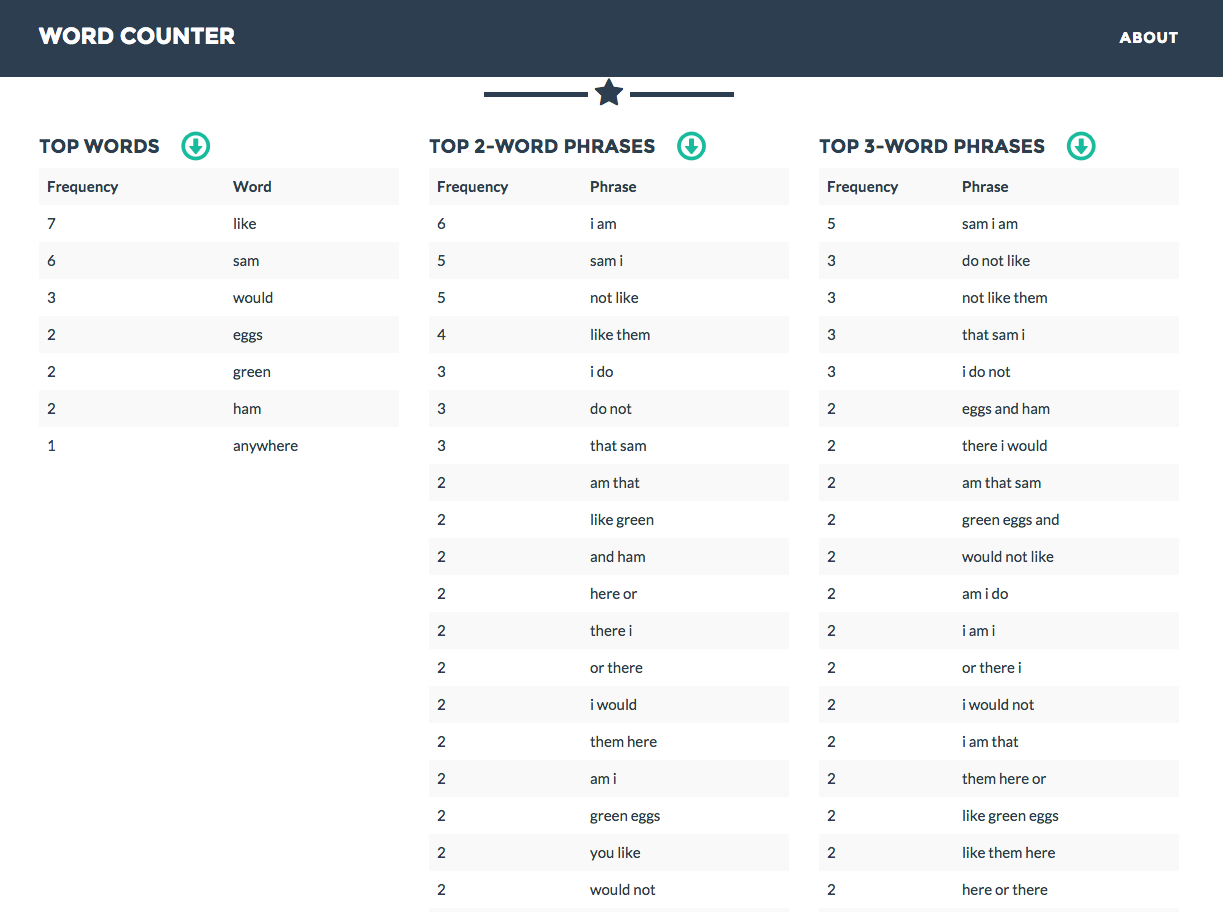
\includegraphics[width=\linewidth]{wordcounterresults}
\label{fig:wordcounterresults}
\end{figure}

\subsection{An Activity to Analyze Music Lyrics}

To introduce WordCounter and text mining concepts to the students we used corpora from song lyrics. This builds on a rich tradition of analyzing music lyrics as data \cite{wattenberg_arc_2002,hemphill_rap_2014}. We used available archives to create lyrical corpora for a variety of popular musical artists (Kanye West, Michael Jackson, the Beatles, Elvis Presley, Nicki Minaj, etc.) and provided them to students. Working in groups of three, students had twenty minutes to decide which lyrics to run through WordCounter in order to find a story to tell with the results. This built on prior classes in our syllabi that had addressed exploratory data analysis as a story-finding process. Students used markers and large pads of paper to create a sketch of a visual presentation of their story to share with peers for feedback. The class spent 10-15 minutes discussing the stories and using them as a jumping off point for further discussion of text mining and text analysis concepts. 

\section{Discussion}

We evaluated this example tool and activity in terms of how it fulfills our design principles, and also how it helps build our definition of core data literacy skills in learners.

\subsection{Implementing Our Design Principles}

WordCounter fulfills the design principles that we defined above for data literacy learning tools. It is \textbf{\textit{focused}} on the technical task of counting word frequency in unstructured text. There is a single point of input and single point of output, which is to say its scope is purposefully limited. This provides a fairly low entry point.  It is strongly \textbf{\textit{guided}} by the activity using song lyrics. In addition, at first load it offers an excerpt from Dr. Seuss' classic \emph{Green Eggs and Ham} as sample text to try the tool with.  WordCounter is \textbf{\textit{inviting}} to learners because of its bold text, clean design, playful naming and example text. Our activity design reinforces this through the use of popular music lyrics, and markers and large paper as the output for sketching stories.  Referring back to our pedagogical themes, the choice to use music lyrics is our intentional attempt to put Freire's concept of \emph{generative themes} into practice - music lyrics have traditionally embodied and reflected the main themes contemporary society is struggling with. WordCounter is \textbf{\textit{expandable}} by starting with a simple concept, counting word frequency, but including links to download CSVs for further analysis in other, more sophisticated, tools. In addition, our copy-writing reinforces this using descriptions such as \enquote{two word phrases (bigrams)} to explain an aspect in both novice and technical language.  The activity reinforces this with a facilitated discussion after the project sharing that touches on concepts that invariably come up with the sketches such as stopwords, stemming and normalization across corpora of various sizes.

\subsection{Building Data Literacy}

\begin{figure}[h]
\caption{Student comparison of the lyrics of Paul Simon and Kanye West. Notably, they converge on \enquote{La la la}.}
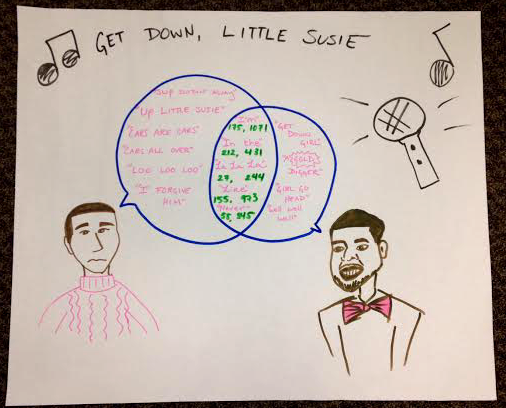
\includegraphics[width=\linewidth]{KanyePaulSimon}
\label{fig:KanyePaulSimon}
\end{figure}

We used WordCounter and the accompanying lyrics analysis activity with two sets of undergraduate and graduate learners in data storytelling courses. One group included undergraduate journalism majors, while the other included students from a mix of degree programs at both undergraduate and graduate levels. Figure \ref{fig:KanyePaulSimon} shows a typical student presentation. This group of students chose to compare the lyrics of Paul Simon and Kanye West, finding that they converged on terms like \enquote{I'm} and \enquote{La la la}. Many students chose to compare the lyrics of two or more artists and represent their similarities and differences in some way. Figure \ref{fig:narcissism} shows a group that tried to determine which artist was the most narcissistic based on how many times they mentioned themselves. Other groups used the data as input for a generative creative process; for example one group wrote a new song with the most common words from ten artists' corpora. 

\begin{figure}[h]
\caption{Student measurement of how often various artists mention themselves.}
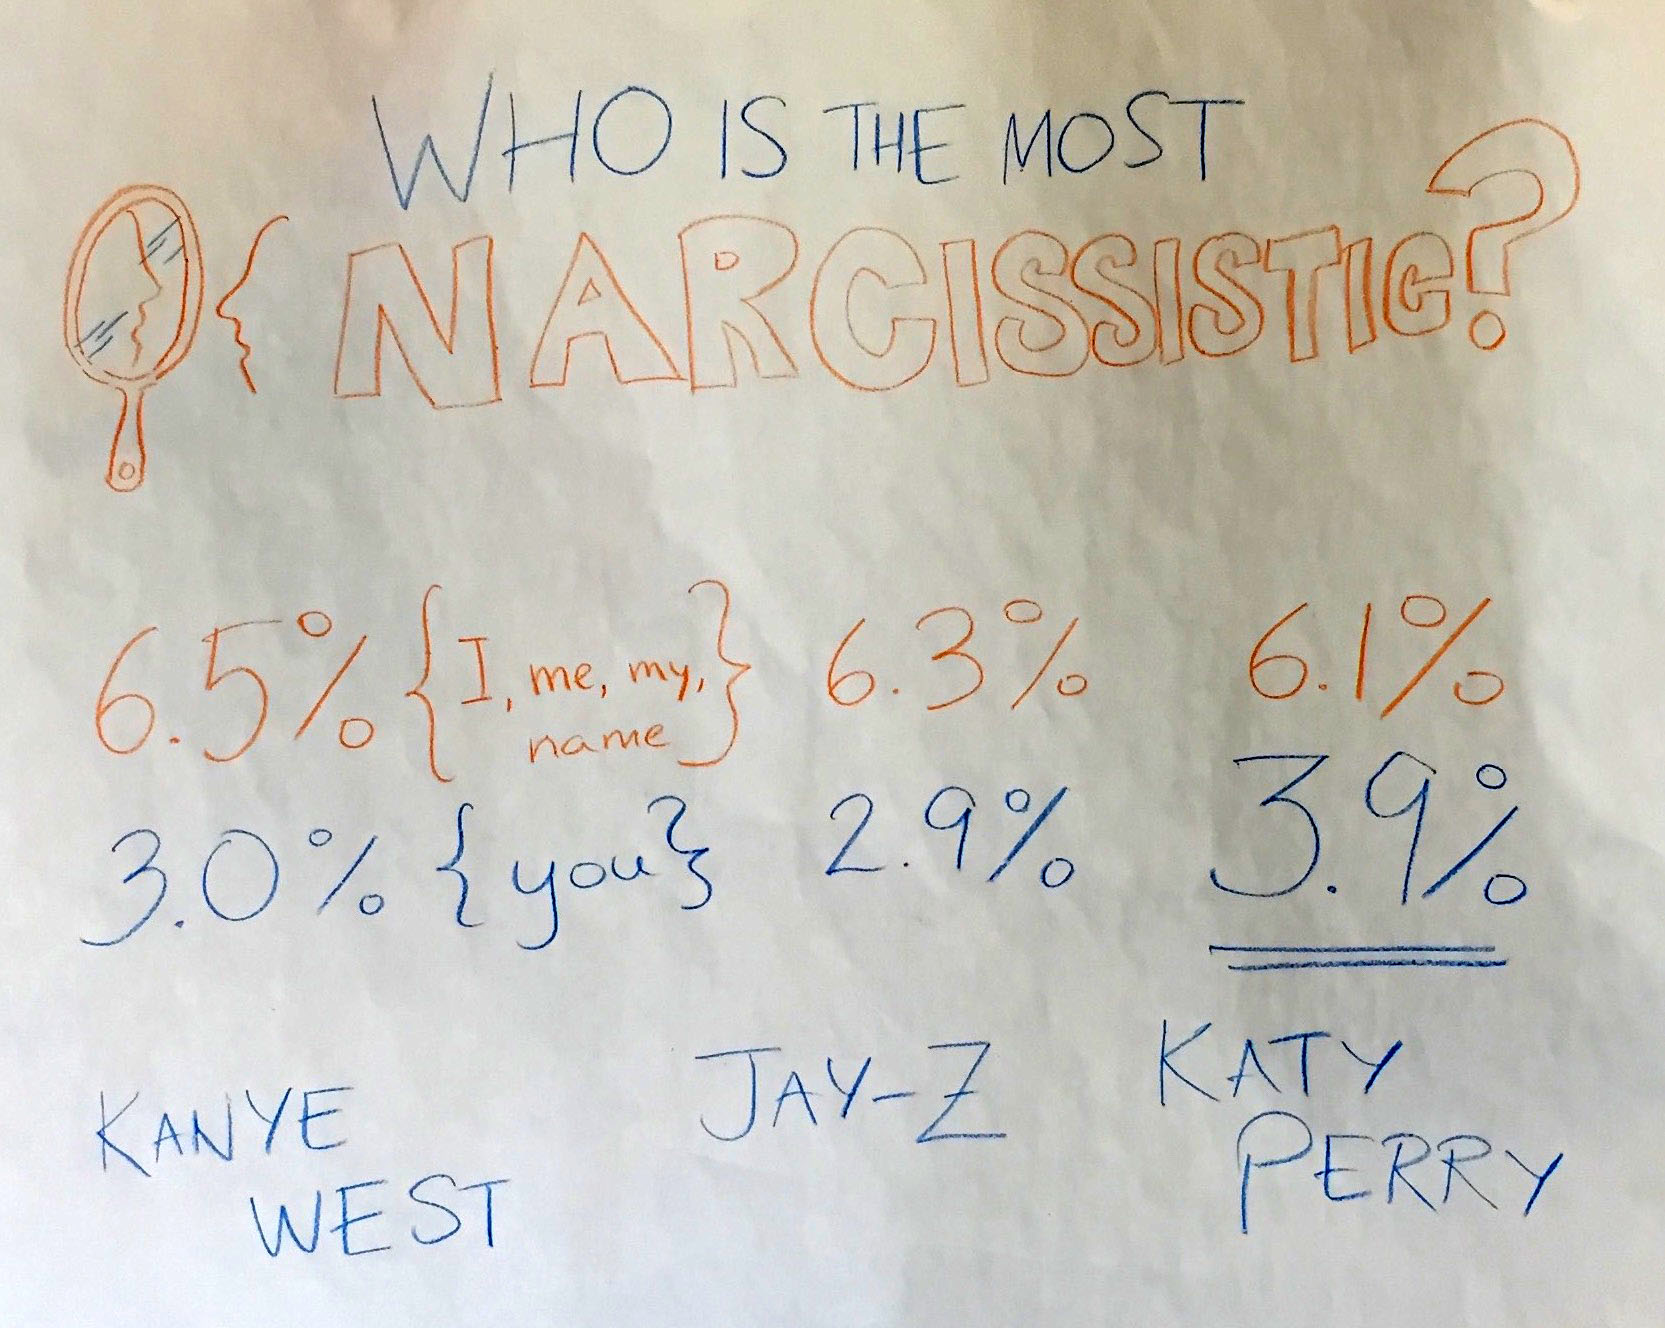
\includegraphics[width=\linewidth]{narcissism}
\label{fig:narcissism}
\end{figure}

These sketches are informal visual presentations that demonstrate students' learning outcomes. They embody the students' ability to read, work with, analyze and argue with data. Students \textbf{\textit{read}} word frequency counts in order to understand patterns in the lyrics of each artist. They \textbf{\textit{worked with}} the data by discussing ideas, running WordCounter on different corpora, and making multiple sketches of their final visual presentation. Students \textbf{\textit{analyzed}} data by looking at multiple groups of song lyrics or by looking for the occurrence of specific words (like \enquote{time}, \enquote{me} or \enquote{La la la}) within an artist's lyrics.  Students \textbf{\textit{argued}} with data by presenting their final story to the class and hearing feedback on their analysis and visual presentation.

This case presents a first pass at implementing the design principles we proposed for tools that are built for data literacy learners.  While just a prototype, it strongly suggests that following these principles can achieve outcomes that increase data literacy along the axes we have defined.  There are certainly opportunities to expand this tool and activity to be further aligned with our design principles.  For instance, our activity is specifically designed for the classroom setting, while the web-based tool itself could be discovered and used in any setting.  There are design opportunities to fold in self-paced activities or tutorials more thoroughly into the tool itself to facilitate reflection, critical thinking, and further learning (as per our pedagogical principles).

\section{Conclusion}

The proliferation of data tools created in response to the growing demand from novices to work with data is missing an opportunity to better support data literacy learners.  Building data literacy requires tool builders to think about their audience as \emph{learners} rather than users. We urge designers and educators to approach their tools and activities with learners in mind, rather than focusing on the outputs the tools create. For educators, these design principles offer a set of criteria for evaluating tools to use in classrooms or other instructional settings. For tool designers, these design principles offer a template for features that should be included and excluded from the simplest versions of your tools. This pedagogical re-alignment is fundamental to helping build a stronger support system for data literacy learners.

\bibliographystyle{abbrv}
\bibliography{data-literacy}

%\balancecolumns 

\end{document}
